%---------------------------------------------------------------------------%
%-                                                                         -%
%-                           LaTeX Template                                -%
%-                                                                         -%
%---------------------------------------------------------------------------%
%- Copyright (C) Huangrui Mo <huangrui.mo@gmail.com> 
%- This is free software: you can redistribute it and/or modify it
%- under the terms of the GNU General Public License as published by
%- the Free Software Foundation, either version 3 of the License, or
%- (at your option) any later version.
%---------------------------------------------------------------------------%
%->> Document class declaration
%---------------------------------------------------------------------------%
\documentclass[twoside]{Style/uwaterloothesis}%
%- Multiple optional arguments:
%- [<oneside|twoside|print>]% oneside eprint, twoside eprint, or paper print
%- [draftversion]% show draft version information
%- [standard options for book class: draft|paper size|font size|...]%
%---------------------------------------------------------------------------%
%->> Document settings
%---------------------------------------------------------------------------%
\usepackage[list]{Style/artratex}% document settings
%- usage: \usepackage[option1,option2,...,optionN]{artratex}
%- Multiple optional arguments:
%- [bibtex|biber]% set bibliography processor and package
%- [<numbers|super|authoryear|alpha>]% set citation and reference style
%- <numbers>: textual: Jones [1]; parenthetical: [1]
%- <super>: textual: Jones superscript [1]; parenthetical: superscript [1]
%- <authoryear>: textual: Jones (1995); parenthetical: (Jones, 1995)
%- <alpha>: textual: not available; parenthetical: [Jon95]
%- [geometry]% reconfigure page layout via geometry package
%- [lscape]% provide landscape layout environment
%- [xhf]% disable header and footer via fancyhdr package
%- [color]% provide color support via xcolor package
%- [background]% enable page background
%- [tikz]% provide complex diagrams via tikz package
%- [table]% provide complex tables via ctable package
%- [list]% provide enhanced list environments for algorithm and coding
%- [math]% enable some extra math packages
%- [xlink]% disable link colors
\usepackage{Style/artracom}% user defined commands
%---------------------------------------------------------------------------%
%->> Document inclusion
%---------------------------------------------------------------------------%
%\includeonly{Tex/Chap_1,...,Tex/Chap_N}% selected files compilation
%---------------------------------------------------------------------------%
%->> Document content
%---------------------------------------------------------------------------%
%-
%-> Titlepage information
%-
%---------------------------------------------------------------------------%
%->> Titlepage information
%---------------------------------------------------------------------------%
\title[\LaTeX{} Thesis Template of UW]{\LaTeX{} Thesis Template\\ of\\ The University of Waterloo}% \title[short title for headers]{Long title of thesis}
\author{Huangrui Mo}
\degree{Doctor of Philosophy}
\discipline{Mechanical and Mechatronics Engineering}
%---------------------------------------------------------------------------%
%
\begin{document}
%-
%-> Frontmatter: title page, abstract, content list, symbol list, preface
%-
\frontmatter% initialize the environment
%---------------------------------------------------------------------------%
%->> Frontmatter
%---------------------------------------------------------------------------%
%-
%-> Titlepage
%-
\maketitle
%-
%-> Examining Committee Membership
%-
\intotoc*{\cleardoublepage}{Examining Committee Membership}% add link to toc
\begin{committee}
    \noindent
    The following served on the Examining Committee for this thesis. The decision of the Examining Committee is by majority vote.

    \begin{center}
        %\footnotesize% fontsize
        \setlength{\tabcolsep}{10pt}% column separation
        \renewcommand{\arraystretch}{3}% row space 
        \begin{tabular}{lc}
            External Examiner & \parbox[t]{10cm}{Dr. Luc Bauwens\\Professor, Mechanical and Manufacturing Engineering\\University of 
Calgary}\\
            Supervisors & \parbox[t]{10cm}{Dr. Fue-Sang Lien\\Professor, Mechanical and Mechatronics Engineering\\University of Waterloo}\\
             & \parbox[t]{10cm}{Dr. Fan Zhang\\Senior Scientist, Advanced Energetics Group\\Defence Research and Development Canada}\\
             & \parbox[t]{10cm}{Dr. Duane Cronin\\Professor, Mechanical and Mechatronics Engineering\\University of Waterloo}\\
            Internal Members & \parbox[t]{10cm}{Dr. Cecile Devaud\\Professor, Mechanical and Mechatronics Engineering\\University of Waterloo}\\
             & \parbox[t]{10cm}{Dr. Jean-Pierre Hickey\\Professor, Mechanical and Mechatronics Engineering\\University of Waterloo}\\
            Internal-External Member & \parbox[t]{10cm}{Dr. Lilia Krivodonova\\Professor, Applied Mathematics\\University of Waterloo}\\
        \end{tabular}
    \end{center}
\end{committee}
%-
%-> Author's declaration
%-
\intotoc*{\cleardoublepage}{Author's Declaration}% add link to toc
\begin{declaration}
    \noindent
    I hereby declare that I am the sole author of this thesis. This is a true copy of the thesis, including any required final revisions, as accepted by my examiners.

    \bigskip

    \noindent
    I understand that my thesis may be made electronically available to the public.
\end{declaration}
%-
%-> Statement of Contributions
%-
%\intotoc*{\cleardoublepage}{Statement of Contributions}% add link to toc
%\begin{contribute}
%\end{contribute}
%-
%-> Permissions
%-
%\intotoc*{\cleardoublepage}{Permissions}% add link to toc
%\begin{permission}
%    \noindent
%\end{permission}
%-
%-> Abstract
%-
\intotoc*{\cleardoublepage}{Abstract}% add link to toc
\begin{abstract}
    This is a short brochure on how to write your thesis by using this \LaTeX{} template. It's easy, efficient and straightforward. What you need to do, no matter you are familiar with \LaTeX{} or not, is to have a try.
\end{abstract}
%-
%-> Acknowledgements
%-
\intotoc*{\cleardoublepage}{Acknowledgements}% add link to toc
\begin{acknowledgements}

    I owe my deepest gratitude and appreciation to my doctoral advisors: Dr. Fue-Sang Lien, Dr. Fan Zhang, and Dr. Duane Cronin. Dr. Fue-Sang Lien has always been supportive, approachable, and helpful throughout my doctoral study. His encouragement and understanding helped me go through the difficulties and created the space for me to develop research ideas. Working with Dr. Fan Zhang has been the most amazing experience in my life. I have always been fascinated by his insights on physics and the ability to instantly and accurately identify the key problems based on a set of fragmented information. His keen and open-minded guidance inspired my interests in the field of my doctoral study, shaped my critical thinking, and challenged me to be a higher level thinker. It was an enlightening and enriching experience to collaborate with Dr. Duane Cronin. Whenever I needed advice, he was ready and patient to help. He was always kind to teach me and willing to share his experience and vision on how to be a professional, rigorous, and persuasive researcher. The moments I interacted with and the knowledge I learned from my outstanding advisors will be remembered by me throughout the rest of my life.

    I am grateful to Natural Sciences and Engineering Research Council of Canada (NSERC), Defence Research and Development Canada (DRDC), and Waterloo CFD Engineering Consulting Inc (WATCFD) for the financial support of this research project. This work was made possible by the facilities of the Shared Hierarchical Academic Research Computing Network (SHARCNET: www.sharcnet.ca) and Compute/Calcul Canada.

    I would like to thank the official members of my examining committee for their efforts in reviewing my thesis and providing helpful suggestions. In addition, I want to express my gratitude to Dr. Jean-Pierre Hickey for his kind help with my teaching practice, to Dr. Cecile Devaud for her helpful comments on my comprehensive examination report, to Dr. Lilia Krivodonova for her thoughtful teaching on numerical solutions of partial differential equations, and to Dr. Luc Bauwens for taking his time to come and attend my examination in person. I also want to thank my colleagues in the Energy Research Center for their support and discussions and the faculty and staff in the Mechanical and Mechatronics Engineering department for their assistance and help throughout my doctoral study. Finally, I am indebted to my family for their continuous support and understanding with my pursuit of scientific research.

\end{acknowledgements}
%-
%-> Dedication
%-
%\intotoc*{\cleardoublepage}{Dedication}% add link to toc
%\begin{dedication}
%    Dedication (included if necessary)
%\end{dedication}
%---------------------------------------------------------------------------%
% title page, abstract
{% content list region
\linespread{1.1}% local line space
\intotoc*{\cleardoublepage}{\contentsname}% add link to bookmark
\tableofcontents% content catalog
\intotoc*{\cleardoublepage}{\listfigurename}% add link to bookmark
\listoffigures% figure catalog
\intotoc*{\cleardoublepage}{\listtablename}% add link to bookmark
\listoftables% table catalog
}
%%
%% >>> Nomenclatures
%%
\intotoc\chapter*{Nomenclature}

\section*{Characters}
\nomenclatureitem[\textbf{Unit}]{\textbf{Symbol}}{\textbf{Description}}
\nomenclatureitem[$\Unit{m^{2} \cdot s^{-2} \cdot K^{-1}}$]{$R$}{specific gas constant}
\nomenclatureitem[$\Unit{m^{2} \cdot s^{-2} \cdot K^{-1}}$]{$C_v$}{specific heat capacity at constant volume}
\nomenclatureitem[$\Unit{m^{2} \cdot s^{-2} \cdot K^{-1}}$]{$C_p$}{specific heat capacity at constant pressure}
\nomenclatureitem[$\Unit{m^{2} \cdot s^{-2}}$]{$e_{\Des{T}}$}{specific total energy}
\nomenclatureitem[$\Unit{m^{2} \cdot s^{-2}}$]{$e$}{specific internal energy}
\nomenclatureitem[$\Unit{m^{2} \cdot s^{-2}}$]{$h_{\Des{T}}$}{specific total enthalpy}
\nomenclatureitem[$\Unit{m^{2} \cdot s^{-2}}$]{$h$}{specific enthalpy}
\nomenclatureitem[$\Unit{kg \cdot m \cdot s^{-3} \cdot K^{-1}}$]{$k$}{thermal conductivity}
\nomenclatureitem[$\Unit{K}$]{$T$}{temperature}
\nomenclatureitem[$\Unit{s}$]{$t$}{time}
\nomenclatureitem[$\Unit{kg \cdot m^{-1} \cdot s^{-2}}$]{$p$}{thermodynamic pressure}
\nomenclatureitem[$\Unit{kg \cdot m^{-1} \cdot s^{-2}}$]{$\hat{p}$}{hydrostatic pressure}
\nomenclatureitem[$\Unit{kg \cdot m^{-2} \cdot s^{-2}}$]{$\Vector{f}_{\Des{b}}$}{body force}
\nomenclatureitem[$\Unit{m^2}$]{$S$}{boundary surface}
\nomenclatureitem[$\Unit{m^3}$]{$\Omega$}{spatial domain}
\nomenclatureitem[$\Unit{m \cdot s^{-1}}$]{$\Vector{V}$}{velocity vector}
\nomenclatureitem[$\Unit{m \cdot s^{-1}}$]{$u$}{x component of velocity}
\nomenclatureitem[$\Unit{m \cdot s^{-1}}$]{$v$}{y component of velocity}
\nomenclatureitem[$\Unit{m \cdot s^{-1}}$]{$w$}{z component of velocity}
\nomenclatureitem[$\Unit{m \cdot s^{-1}}$]{$c$}{speed of sound}
\nomenclatureitem[$\Unit{m}$]{$\Vector{x}$}{position vector}
\nomenclatureitem[$\Unit{1}$]{$\unitVector{n}$}{unit outward normal vector}
\nomenclatureitem[$\Unit{1}$]{$\hat{\unitVector{t}}$}{unit tangent vector}
\nomenclatureitem[$\Unit{1}$]{$\tilde{\unitVector{t}}$}{unit bitangent vector}
\nomenclatureitem[$\Unit{1}$]{$C_{\Des{R}}$}{coefficient of restitution}
\nomenclatureitem[$\Unit{1}$]{$Re$}{Reynolds number}
\nomenclatureitem[$\Unit{1}$]{$Pr$}{Prandtl number}
\nomenclatureitem[$\Unit{1}$]{$Ma$}{Mach number}
\nomenclatureitem[$\Unit{m^2 \cdot s^{-1}}$]{$\alpha$}{thermal diffusivity}
\nomenclatureitem[$\Unit{kg \cdot m^{-1} \cdot s^{-1}}$]{$\mu$}{dynamic viscosity}
\nomenclatureitem[$\Unit{m^2 \cdot s^{-1}}$]{$\nu$}{kinematic viscosity}
\nomenclatureitem[$\Unit{1}$]{$\gamma$}{heat capacity ratio}
\nomenclatureitem[$\Unit{kg \cdot m^{-3}}$]{$\rho$}{density}
\nomenclatureitem{$\Vector{U}$}{vector of conservative variables}
\nomenclatureitem{$\Vector{F}$}{vector of fluxes}
\nomenclatureitem{$\Vector{\Phi}$}{vector of source terms}
\nomenclatureitem[$\Unit{kg \cdot m^{-1} \cdot s^{-2}}$]{$\Tensor{\sigma}$}{stress tensor}
\nomenclatureitem[$\Unit{kg \cdot m^{-1} \cdot s^{-2}}$]{$\Tensor{S}$}{deviatoric stress tensor}
\nomenclatureitem[$\Unit{kg \cdot m^{-1} \cdot s^{-2}}$]{$\Tensor{\tau}$}{viscous stress tensor}
\nomenclatureitem[$\Unit{1}$]{$\Tensor{\delta}$}{Kronecker tensor}
\nomenclatureitem[$\Unit{1}$]{$\unitTensor{I}$}{identity tensor}

\section*{Operators}
\nomenclatureitem{\textbf{Symbol}}{\textbf{Description}}
\nomenclatureitem{$\Order$}{order of magnitude}
\nomenclatureitem{$\Delta$}{difference}
\nomenclatureitem{$\nabla$}{gradient operator}
\nomenclatureitem{$\delta^{\pm}$}{upwind-biased interpolation scheme}
\nomenclatureitem{$\delta^{0}$}{central interpolation scheme}

\section*{Abbreviations}
\nomenclatureitem{\textbf{Acronym}}{\textbf{Description}}
\nomenclatureitem{ANFO}{Ammonium Nitrate Fuel Oil}
\nomenclatureitem{CFD}{Computational Fluid Dynamics}
\nomenclatureitem{CFL}{Courant--Friedrichs--Lewy}
\nomenclatureitem{CJ}{Chapman--Jouguet}
\nomenclatureitem{EOS}{Equation of State}
\nomenclatureitem{JWL}{Jones--Wilkins--Lee}
\nomenclatureitem{TVD}{Total Variation Diminishing}
\nomenclatureitem{SSP}{Strong Stability Preserving}
\nomenclatureitem{WENO}{Weighted Essentially Non-oscillatory}
\nomenclatureitem{ZND}{Zel'dovich--von Neumann--Doering}

% symbol list, preface content
%-
%-> Mainmatter
%-
\mainmatter% initialize the environment
%---------------------------------------------------------------------------%
%->> Main content
%---------------------------------------------------------------------------%
\chapter{A Brief Guide}
\label{chap:guide}

\section{What is \LaTeX{}}

\LaTeX{} (pronounced "Lah-tech" or "Lay-tech") is a macro package created by Leslie Lamport based on \TeX{}. As a document preparation system for high-quality typesetting in almost any forms of publishing, \LaTeX{} is not the name of a particular editing program, but refers to the encoding or tagging conventions that are used in \LaTeX{} documents \citep{website:wikipedia,website:latex}. The best resource to learn \LaTeX{} is "\LaTeX{} Wikibook", which is available online.

\section{Why use \LaTeX?}

There are a lot of good reasons why you need to use \LaTeX{}, the most significant one is the following:
\begin{itemize}
    \item Allows you to clearly separate the content from the format of your document.
    \item Let you concentrate on your ideas, not visual appearance.
\end{itemize}

You can concentrate purely on the structure and contents of your document, not superficial layout issues. You don't need to manually adjust fonts, text sizes, line heights, or text flow for readability, as \LaTeX{} takes care of them automatically. \citep{website:wikibook}
\begin{figure}[!htbp]
    \centering
    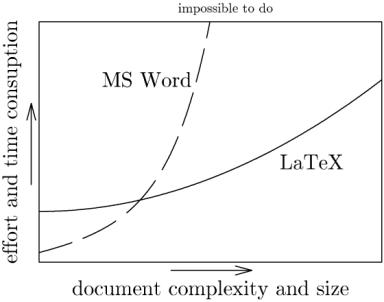
\includegraphics[width=0.6\textwidth]{compare}
    \caption{Comparison between Microsoft Word and \LaTeX{} [From Google Images]}
    \label{fig:compare}
\end{figure}

\section{How to use?}

\subsection{Installation}
LaTeX is based on open-source code, so it is available on most computing platforms as free software. If encounter some compiling problems after installation, please Google it. For example, MikTeX may complain about "mathtools.sty", a solution given on "StackExchange" is "The problem is that the package manager has somehow "desynchronized" (even though it's a fresh install). To fix it, run Miktex Package Manager as administrator---"Package Manager (Admin)". Go to Repository--Synchronize. When that completes, your TexWorks should automatically find the needed style files again."
\begin{itemize}
    \item Linux: TeXLive distribution. 
    \item MacOS: Mactex or TeXLive.
    \item Windows: MikTeX or TeXLive. 
\end{itemize}

Note: to use \LaTeX{}, you need a text editor for writing and editing ".tex" files. To open the ".tex" files in this template, you need a text editor which supports "UTF-8" encoding. Free options for different platforms are the following:
\begin{itemize}
    \item Linux: vim. 
    \item MacOS: TeXShop, Macvim.
    \item Windows: Texmaker, Gvim, Notepad++. 
\end{itemize}

\subsection{Include math}
\LaTeX{} realization of Equation~\ref{eq:appedns} is something like this:
\begin{equation} \label{eq:appedns}
    \begin{cases}
        \frac{\partial \rho}{\partial t} + \nabla\cdot(\rho\Vector{V}) = 0\\
        \frac{\partial (\rho\Vector{V})}{\partial t} + \nabla\cdot(\rho\Vector{V}\Vector{V}) = \nabla\cdot\Tensor{\sigma}\\
        \frac{\partial (\rho E)}{\partial t} + \nabla\cdot(\rho E\Vector{V}) = \nabla\cdot(k\nabla T) + \nabla\cdot(\Tensor{\sigma}\cdot\Vector{V})
    \end{cases}
\end{equation}
\begin{equation}
    \frac{\partial }{\partial t}\int\limits_{\Omega} u \, \mathrm{d}\Omega + \int\limits_{S} \unitVector{n}\cdot(u\Vector{V}) \, \mathrm{d}S = \dot{\phi}
\end{equation}
\[
    \begin{split}
        \mathcal{L} \{f\}(s) &= \int _{0^{-}}^{\infty} f(t) e^{-st} \, \mathrm{d}t, \ 
        \mathscr{L} \{f\}(s) = \int _{0^{-}}^{\infty} f(t) e^{-st} \, \mathrm{d}t\\
        \mathcal{F} {\bigl (} f(x+x_{0}) {\bigr )} &= \mathcal{F} {\bigl (} f(x) {\bigr )} e^{2\pi i\xi x_{0}}, \ 
        \mathscr{F} {\bigl (} f(x+x_{0}) {\bigr )} = \mathscr{F} {\bigl (} f(x) {\bigr )} e^{2\pi i\xi x_{0}}
    \end{split}
\]

mathtext: $A,F,L,2,3,5,\sigma$, mathnormal: $A,F,L,2,3,5,\sigma$, mathrm: $\mathrm{A,F,L,2,3,5,\sigma}$.

mathbf: $\mathbf{A,F,L,2,3,5,\sigma}$, mathit: $\mathit{A,F,L,2,3,5,\sigma}$, mathsf: $\mathsf{A,F,L,2,3,5,\sigma}$.

mathtt: $\mathtt{A,F,L,2,3,5,\sigma}$, mathfrak: $\mathfrak{A,F,L,2,3,5,\sigma}$, mathbb: $\mathbb{A,F,L,2,3,5,\sigma}$.

mathcal: $\mathcal{A,F,L,2,3,5,\sigma}$, mathscr: $\mathscr{A,F,L,2,3,5,\sigma}$, boldsymbol: $\boldsymbol{A,F,L,2,3,5,\sigma}$.

vector: $\Vector{\sigma, T, a, F, n}$, unitvector: $\unitVector{\sigma, T, a, F, n}$

matrix: $\Matrix{\sigma, T, a, F, n}$, unitmatrix: $\unitMatrix{\sigma, T, a, F, n}$

tensor: $\Tensor{\sigma, T, a, F, n}$, unittensor: $\unitTensor{\sigma, T, a, F, n}$ 

\subsection{Include Graphics}
Note: inluding figures may seem to be scary by looking at the codes. However, the fact is that you only need to modify the names in each part, the rest are simply copy and paste. These codes are all available in the file "Useful Commands.txt".

Figure~\ref{fig:oas} is an example for including a single figure.
\begin{center}
    \small
    \begin{verbatim}
        \begin{figure}[!htbp]
            \centering
            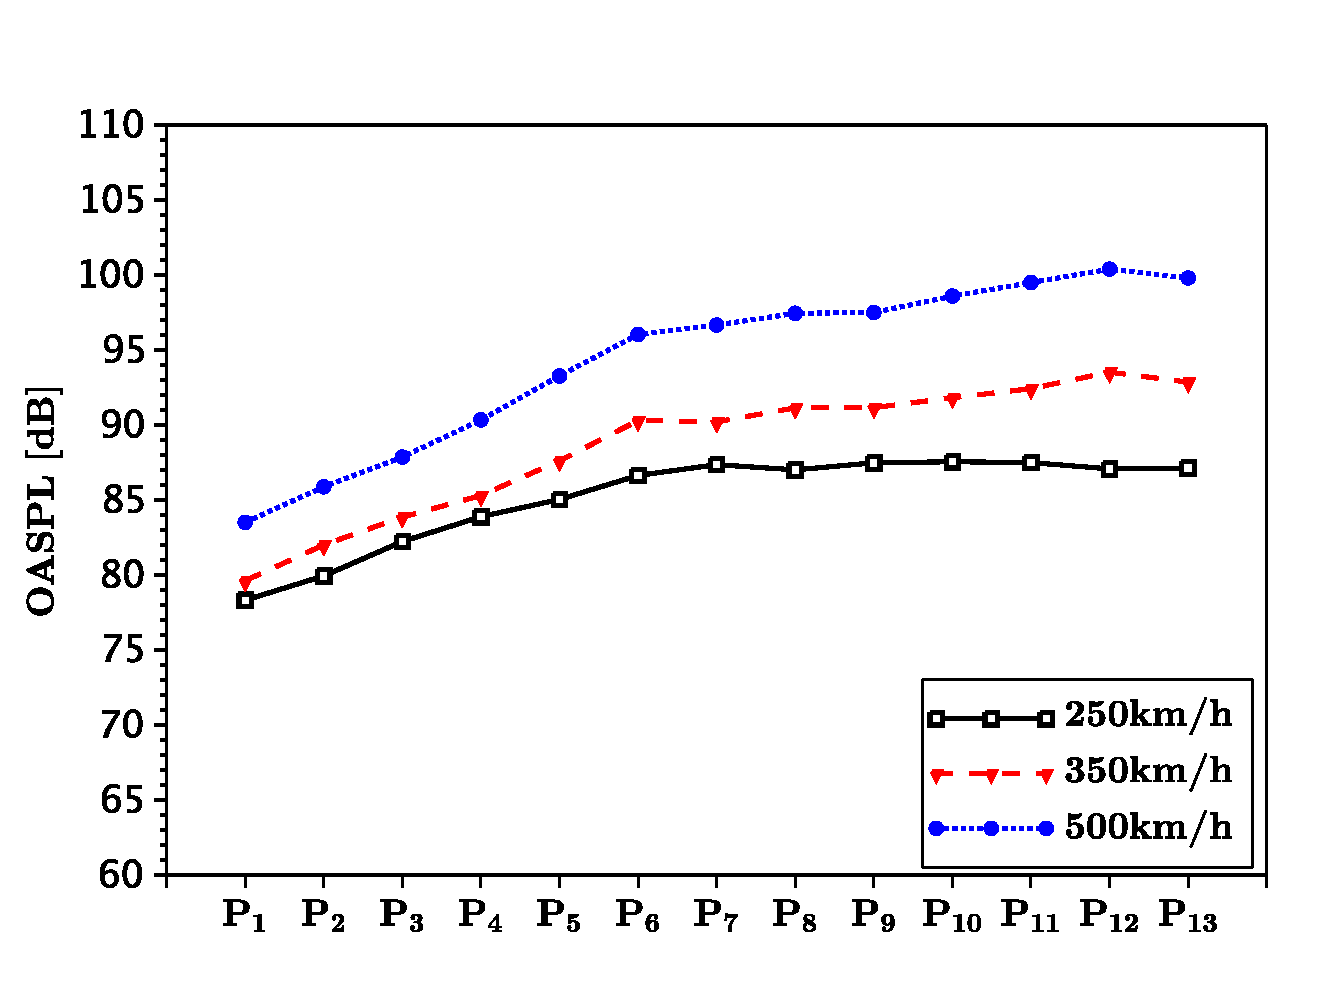
\includegraphics[width=0.45\textwidth]{oaspl_a}
            \caption{An Example for including a single figure}
            \label{fig:oas}
        \end{figure}
    \end{verbatim}
\end{center}

\begin{figure}[!htbp]
    \centering
    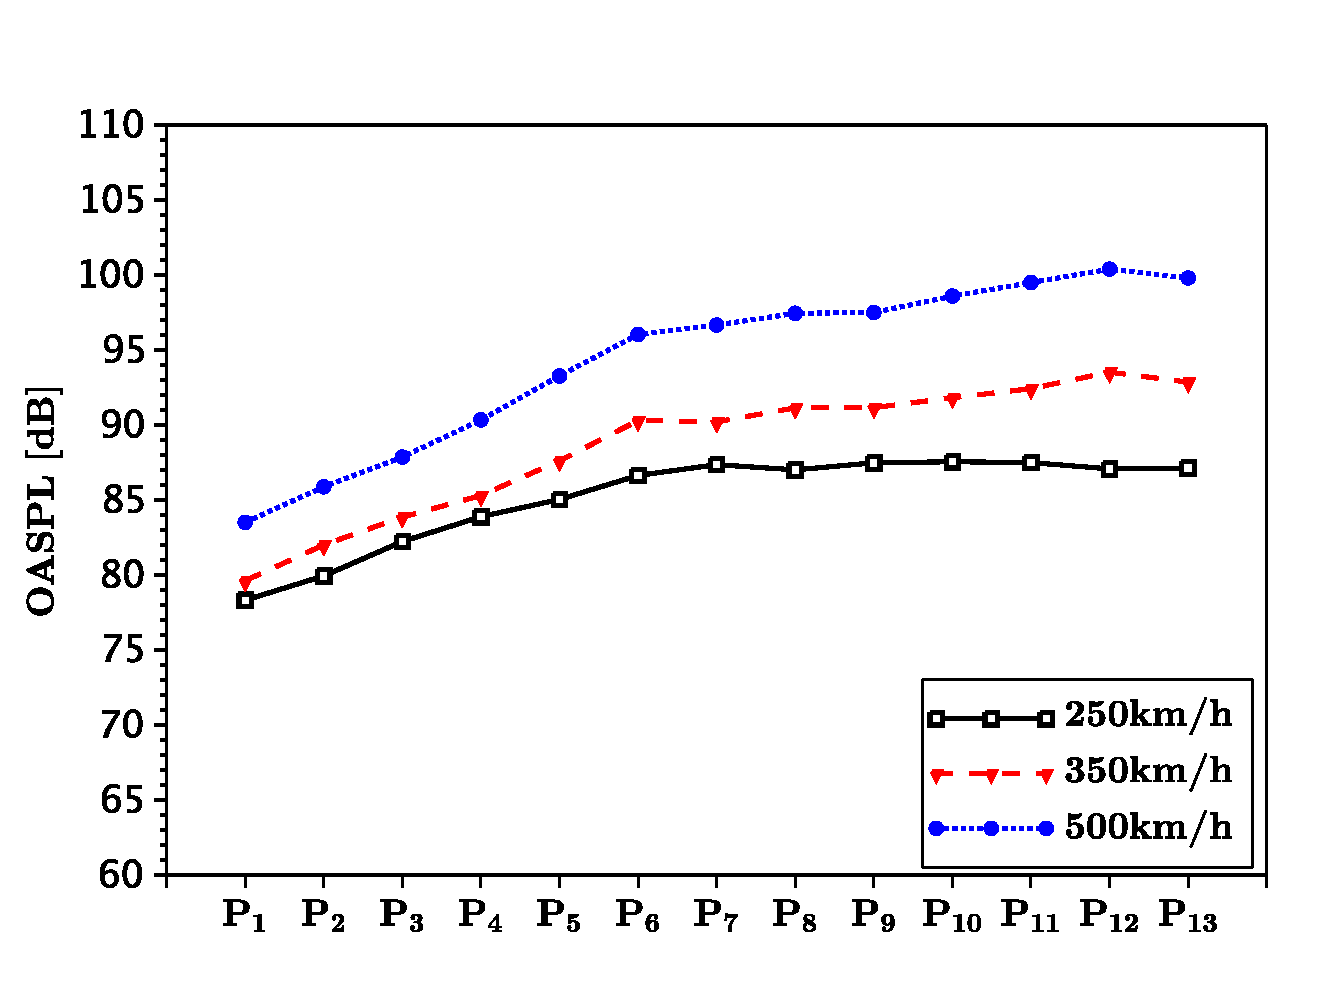
\includegraphics[width=0.45\textwidth]{oaspl_a}
    \caption{An Example for including a single graph}
    \label{fig:oas}
\end{figure}

Figure~\ref{fig:oaspl} is an example for including multiple figuress. 
\begin{center}
    \small
    \begin{verbatim}
        \begin{figure}[!htbp]
            \centering
            \begin{subfigure}[b]{0.45\textwidth}
                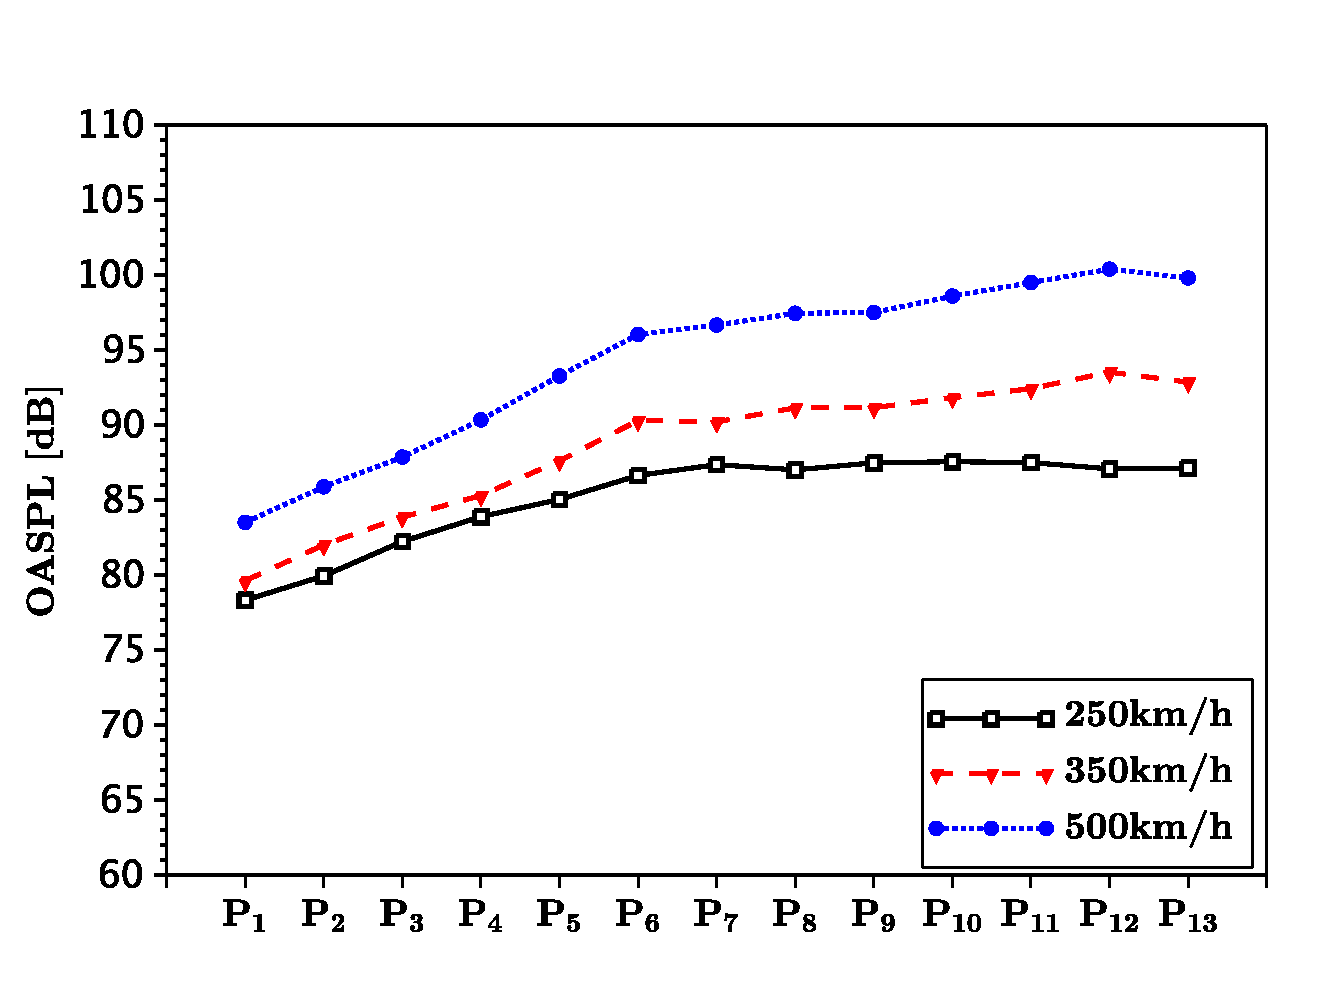
\includegraphics[width=\textwidth]{oaspl_a}
                \caption{}
                \label{fig:oaspl_a}
            \end{subfigure}%
            ~% add a small space
            \begin{subfigure}[b]{0.45\textwidth}
                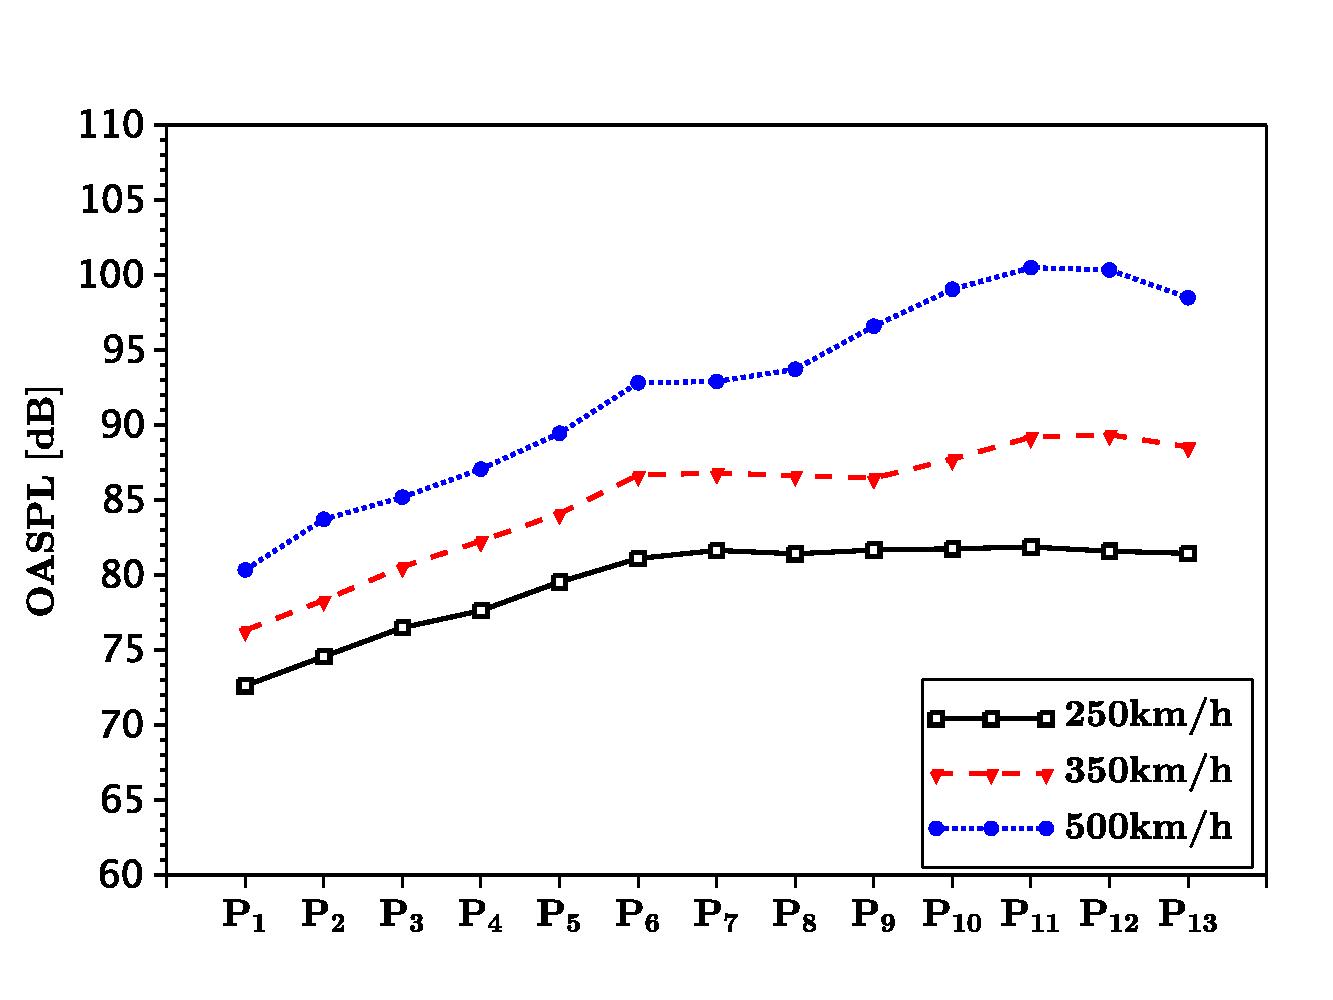
\includegraphics[width=\textwidth]{oaspl_b}
                \caption{}
                \label{fig:oaspl_b}
            \end{subfigure}%
            \\% change line
            \begin{subfigure}[b]{0.45\textwidth}
                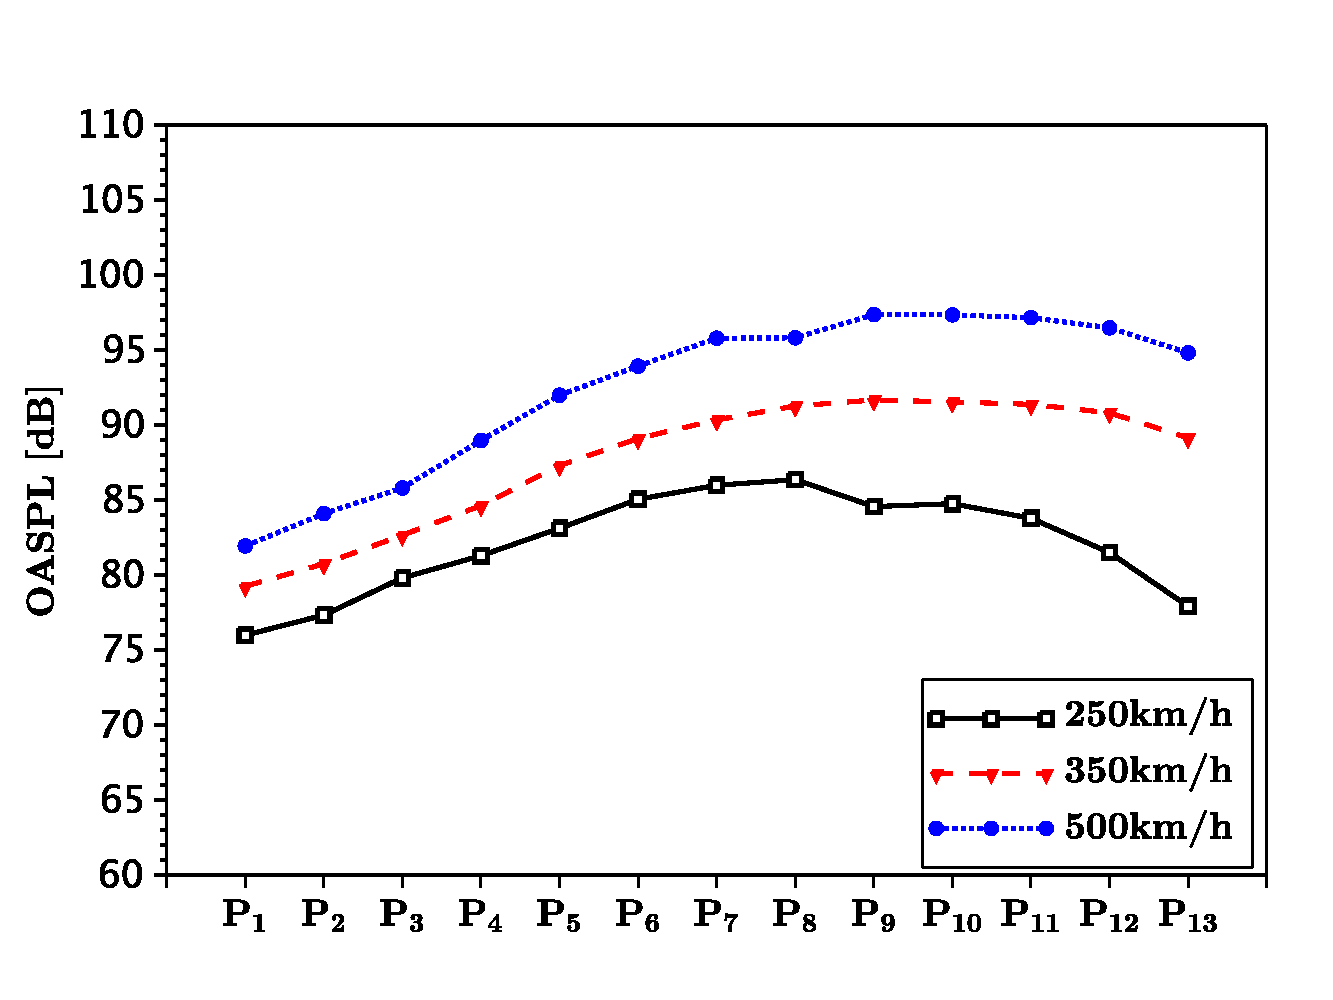
\includegraphics[width=\textwidth]{oaspl_c}
                \caption{}
                \label{fig:oaspl_c}
            \end{subfigure}%
            ~% add a small space
            \begin{subfigure}[b]{0.45\textwidth}
                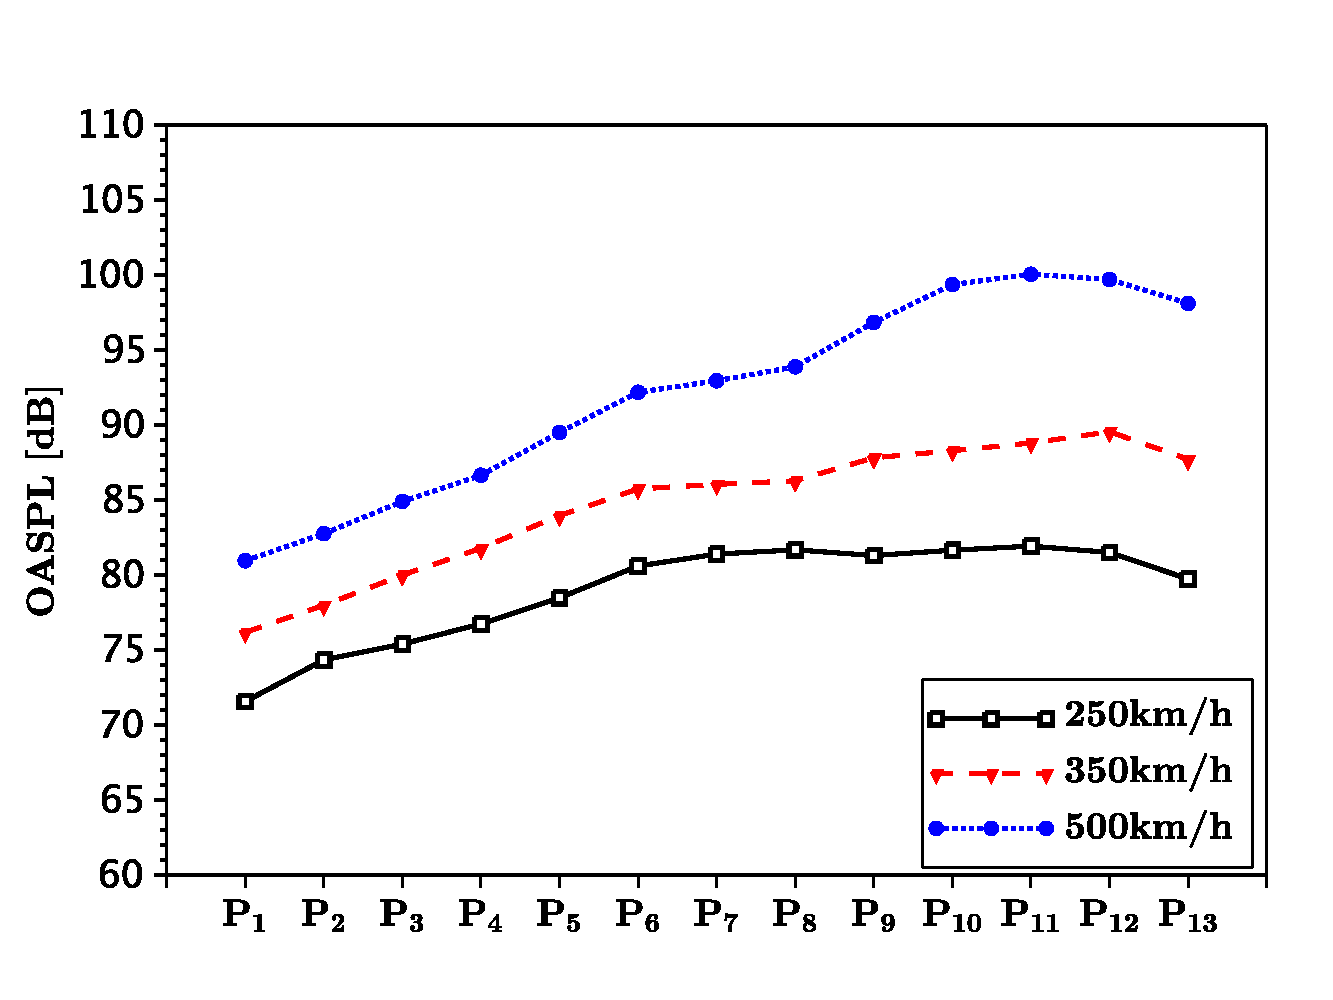
\includegraphics[width=\textwidth]{oaspl_d}
                \caption{}
                \label{fig:oaspl_d}
            \end{subfigure}%
            \caption{An Example for including multiple figures}
            \label{fig:oaspl}
        \end{figure}
    \end{verbatim}
\end{center}
\begin{figure}[!htbp]
    \centering
    \begin{subfigure}[b]{0.45\textwidth}
        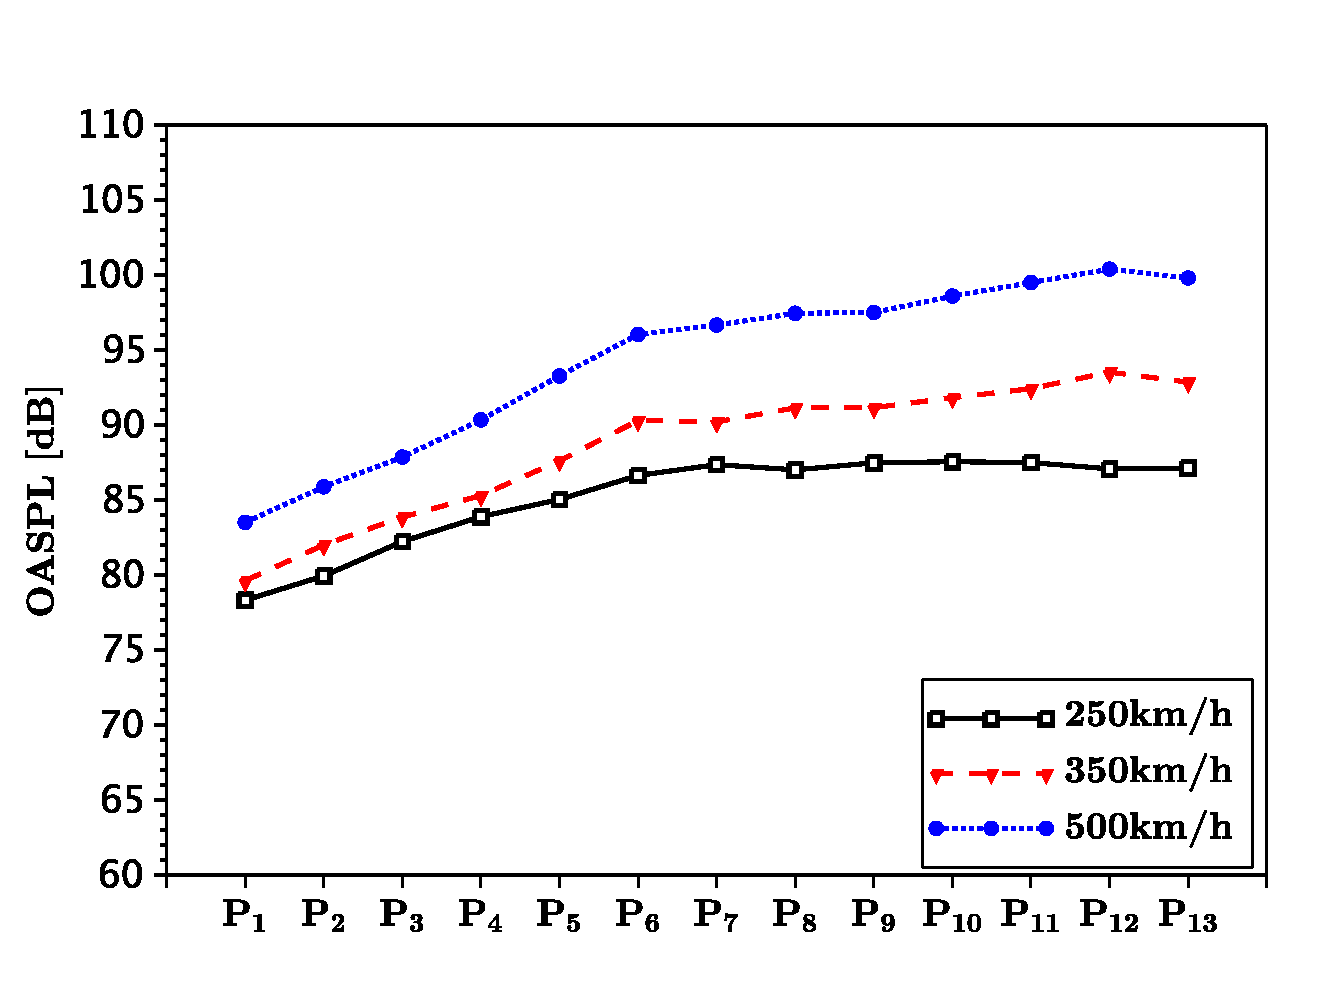
\includegraphics[width=\textwidth]{oaspl_a}
        \caption{}
        \label{fig:oaspl_a}
    \end{subfigure}%
    ~% add a small space
    \begin{subfigure}[b]{0.45\textwidth}
        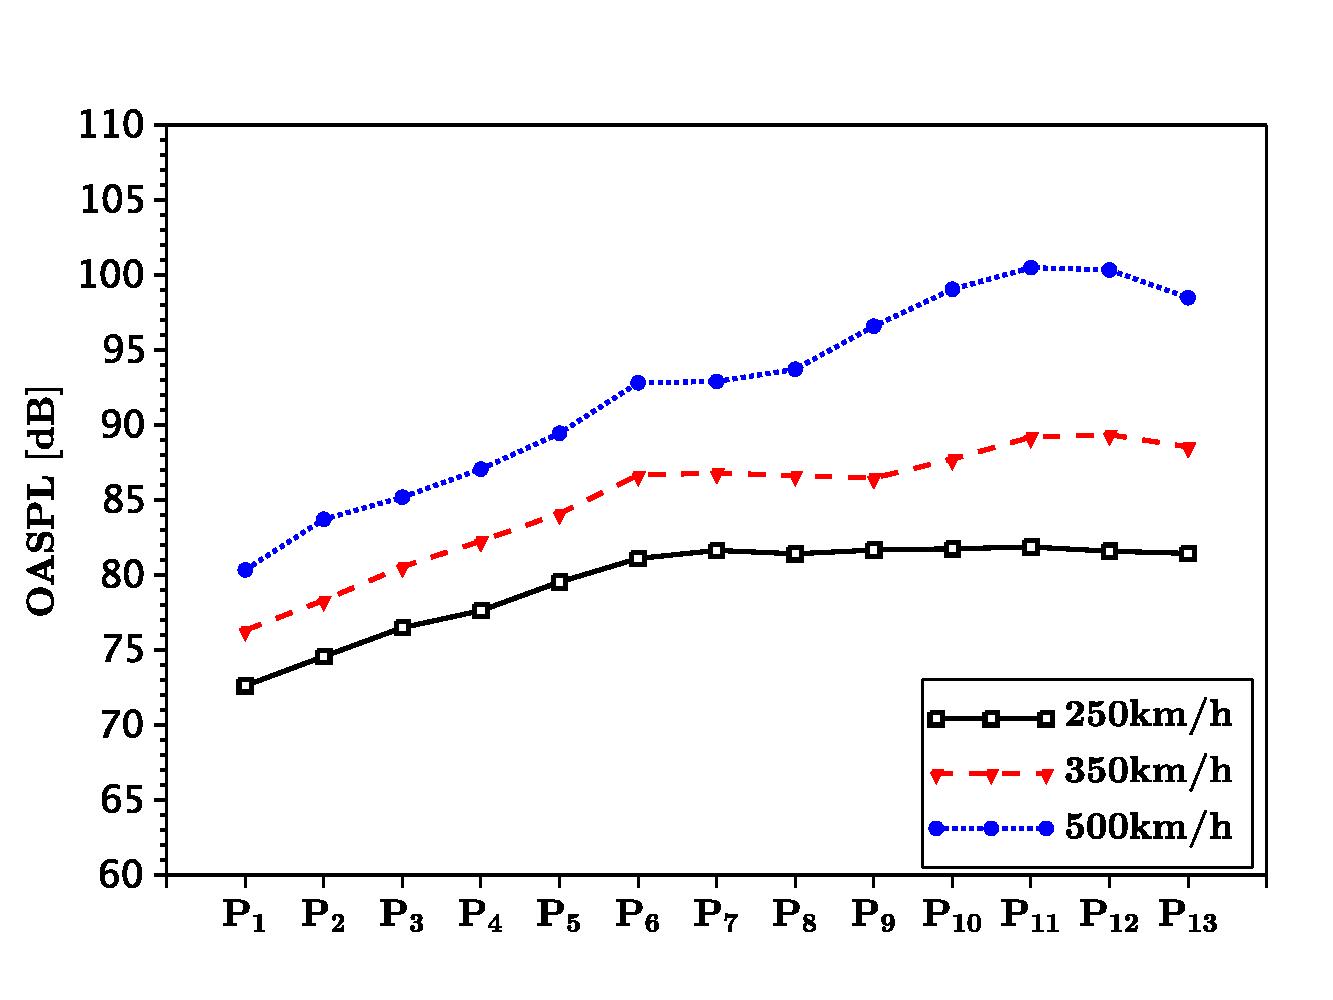
\includegraphics[width=\textwidth]{oaspl_b}
        \caption{}
        \label{fig:oaspl_b}
    \end{subfigure}%
    \\% change line
    \begin{subfigure}[b]{0.45\textwidth}
        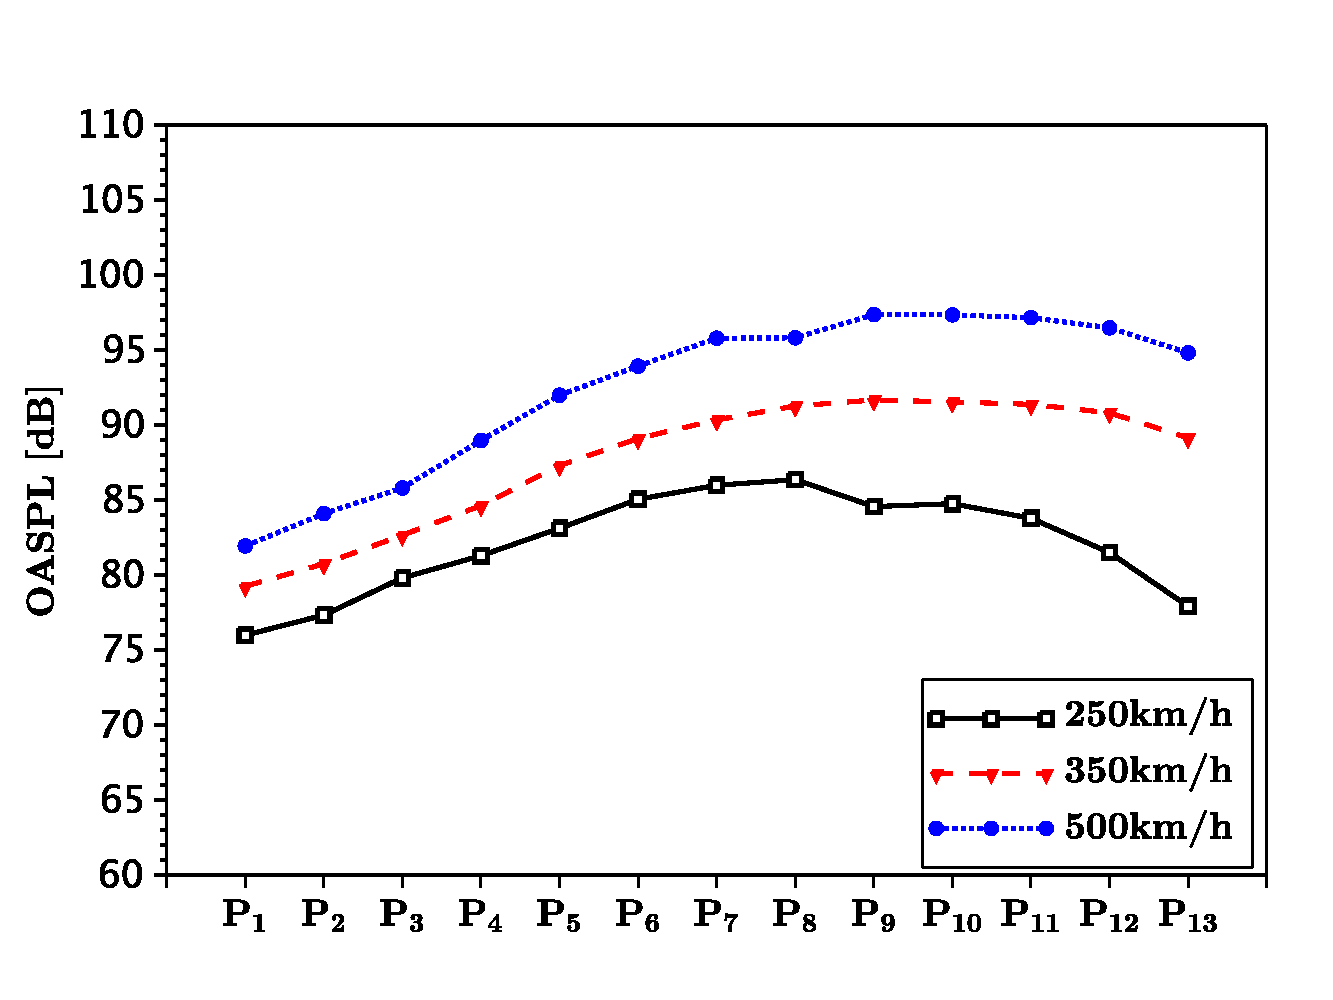
\includegraphics[width=\textwidth]{oaspl_c}
        \caption{}
        \label{fig:oaspl_c}
    \end{subfigure}%
    ~% add a small space
    \begin{subfigure}[b]{0.45\textwidth}
        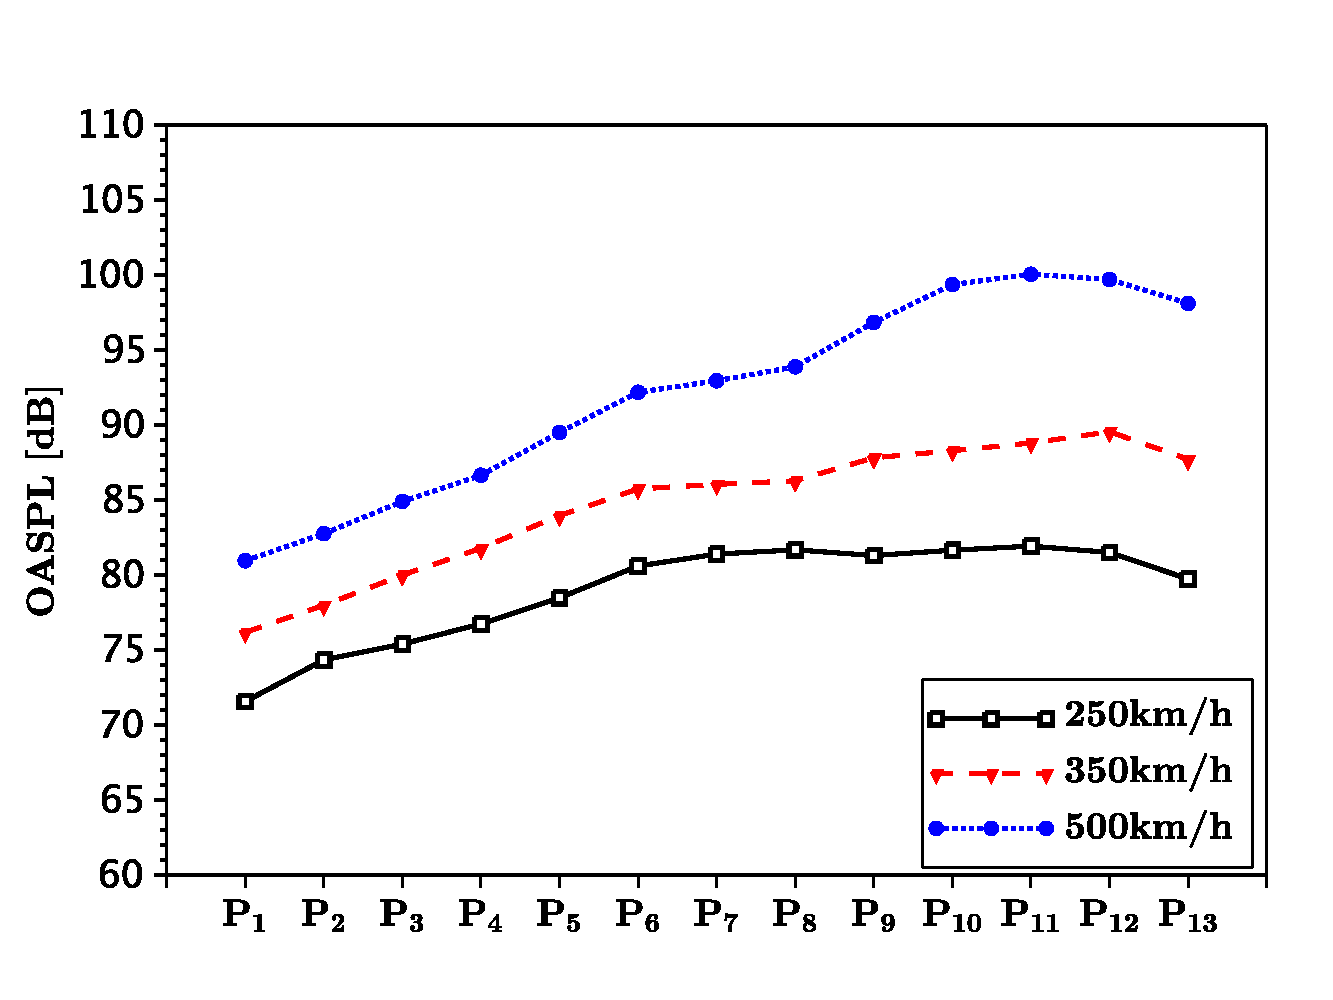
\includegraphics[width=\textwidth]{oaspl_d}
        \caption{}
        \label{fig:oaspl_d}
    \end{subfigure}%
    \caption{An Example for including multiple figures}
    \label{fig:oaspl}
\end{figure}

\subsection{Include a citation}
Suppose you are going to cite an article named "Document Preparation System", the procedures are:
\begin{itemize}
    \item Use Google Scholar search "Document Preparation System".
    \item Open "Cite" and choose "Import to Bibtex" under the target item.
    \item Copy the citation information of this article into the file "Myrefs.bib"
    \item Research dominant: cite this article by \verb+\citep{lamport1986document}+ like here \citep{lamport1986document}
    \item Citation dominant: cite this article by \verb+\citet{lamport1986document}+ like here \citet{lamport1986document}
    \item References list is generated automatically.
\end{itemize}

\subsection{Generate nomenclature}
In this template, a simple command for adding nomenclatures is provided. Therefore, packages for automatical nomenclature generation are not included. From my point of view, there is no need to use those packages and make things complicated. However, if you insist, there are a lot of available packages for creating nomenclatures. Recommended options are (Please Google the one you want to know):
\begin{itemize}
    \item listofsymbols
    \item nomencl
\end{itemize}

\section{File Tree of Current Template}
\begin{itemize}
    \item Thesis.tex: main tex file, which acts like the main function in C++.
    \item Style: Store template configuration files, which act like subfunctions.
    \item Tmp: Store files generated by compilation.
    \item Biblio: Store information of references.
    \item Img: Store images.
    \item Tex: Store files for your content, this is the working directory.
        \begin{itemize}
            \item Frontpages: content of front pages, like authorship, abstract, etc.
            \item Prematter: content of nomenclature, etc.
            \item Main$\_$Content: index for chapters you want to include into your current content.
            \item Chap$\_$***: your content for each chapters.
            \item Appendix: appendix.
            \item Useful Commands: collection of useful commands.
        \end{itemize}
\end{itemize}

Note: this template can be easily adapted to other writing purposes such as articles. What you need to do is to change and adjust a few items in the "Thesis.tex" file, which would be very easy after you are a little familiar with using \LaTeX{}. Like :

Change \verb+\documentclass{uwaterloothesis}+ to \verb+\documentclass{article}+

\section{Feedback and Problems}
Please feel free to send me emails for any related problems:
\begin{center}
huangrui.mo@uwaterloo.ca
\end{center}

%---------------------------------------------------------------------------%
% main content
%-
%-> Appendix
%-
\cleardoublepage%
\appendix% initialize the environment
\chapter{Other Imformation}
% appendix content
%-
%-> Backmatter: bibliography, glossary, index
%-
\backmatter% initialize the environment
\intotoc*{\cleardoublepage}{\bibname}% add link to toc
\bibliography{Biblio/ref}% bibliography
\end{document}
%---------------------------------------------------------------------------%

